\chapter{Introduction to Smith chart}\label{lec:lec7}


\begin{mdframed}[ backgroundcolor=lightblue, linewidth=1pt, hidealllines=true]
\subsection{\textbf{Objectives}}
At the end of this lecture, the student should have a full understanding of:
\begin{enumerate}[(i)]
\item Smith chart's characteristics using the constant reactance and resistance circles
\item Using the Smith chart to solve transmission line analysis and impedance calculation
\item Using normalized impedance and admittance to analyze loads
\item identifying network parameters; maximum and minimum voltage and current, maximum  and minimum resistance using the VSWR circle
\item understand the concept of VSWR circle and movement along the transmission line  using the VSWR cirlce
\item Identifying the types of load from the standing wave pattern: purely reactive loads, purely resistive loads, inductive loads and capacitive loads
\end{enumerate}
\end{mdframed}

\vspace{0.7cm}{Previously, we were able to derive equations for different parameters for a transmission line such as;}
\begin{enumerate}[(i)]
\item Power delivered to the load,
\item Voltage Standing Wave Ratio (VSWR),
\item Maximum and minimum voltage and current,
\item Reflection coefficient,
\item Impedance transformation ratio etc.
\end{enumerate}

Up till now, we analyze transmission line characteristics using \textbf{analytical method}. But in this lecture, we utilize another approach for analyzing the problems of a transmission line which is the \textbf{graphical method}. This approach involves solving the problems of a transmission line from an image called a \textbf{Smith chart}\index{smith chart}. This approach is most preferred for solving transmission line problems than the analytical method owing to the following reasons;
\begin{enumerate}[(i)]
\item Images have a much longer-lasting impression than equations or text on the human mind.
\item The graphical approach is much simpler compared to the analytical approach where calculation can be reduced by significant amount
\item It is a very compact way of representing the impedance characteristics of transmission lines.
\end{enumerate}
So in fact, whenever we are doing transmission line calculation even analytically, it will be appropriate to keep the graphical representation in mind and any analytical method used on transmission line should always be cross checked with the graphical method.
This method if properly understood makes solving transmission line problems much easier and faster. It can also be used as a means of cross-checking the solution obtained using the analytical method so that one does not go conceptually wrong in solving transmission line problems.

It is very important to understand that the graphical method does not give the voltage and current solutions. It gives you only the representation of impedances on the transmission line or the standing wave characteristics of the transmission line. This means it can give you the \textbf{impedance transformation} relationship, and it can give you \textbf{reflection coefficient}, \textbf{VSWR}, location of \textbf{voltage minimum}, location of \textbf{voltage maximum} and so on.
\subsection{Plane Transformation}
In this section, the basic idea is to take the impedance which is normalized with respect to characteristics impedance and do transformation of these impedance into the complex reflection coefficient plane called \textbf{GAMMA}-plane. By doing this then we can transform all impedance from impedance plane to reflection coefficient plane and then we see that this representation of impedances in the reflection coefficient plane makes the calculation much simpler than if we take impedances. The resistive part lies on the real and positive axis and the imaginary part can be positive or negative. Resistance is always real and positive, no negative resistances here. Positive reactance is for inductance and negative reactance for capacitance. So plotting impedance on the complex impedance plane, we get the the diagram below. We saw for the transmission line, what really matter is \index{normalized impedance}. Let us assume our transmission line is lossless. Then the characteristics impedance is a real quantity. All impedance are normalized to the characteristics impedance.
\begin{figure}[h]
\centering
{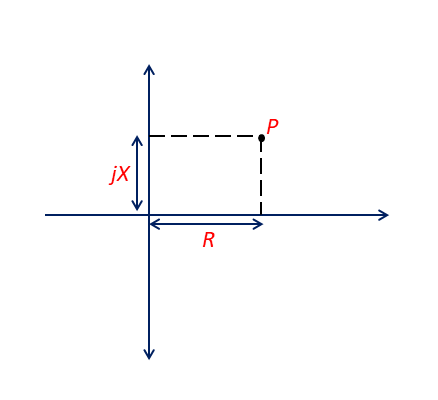
\includegraphics[width=0.8\linewidth]{\pathtopartone/graphics/Z_plane1}}
\caption{Absolute impedance on the complex $Z$-plane}
\label{fig:mjhdj}
\end{figure}

$R$ represents the real part called resistance and $jX$ represents the imaginary part called reactance. Just like in the analytical approach, our analysis using the graphical method will be done with the normalized impedance rather than the \textbf{absolute impedance}. It, therefore, means that, given any impedance, it must be normalized with respect to the characteristic impedance ($Z_0$) such that;
\begin{equation*}
\bar{Z_L}=\frac{Z_L}{Z_0} \quad \text{(normalised)}
\end{equation*}
$Z_L$ is the absolute impedance. So our representation of the normalized impedance would be:
\begin{equation*}
\bar{Z_L}= r + jx
\end{equation*}
Let us represent this expression graphically on the complex z-plane as shown in figure~\ref{fig:transline2}.
\begin{figure}[h]
\center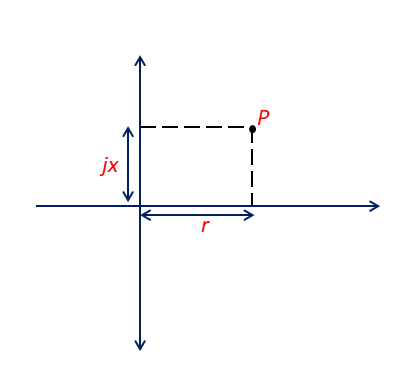
\includegraphics[width=0.8\linewidth]{\pathtopartone/graphics/Zplane}
\caption{Normalized impedance on the complex Z-plane}
\label{fig:transline2}
\end{figure}

From the figure~\ref{fig:transline2}, it is seen that the resistance \textbf{r} is always real and positive. Whereas the reactance could be positive which represents inductive reactance or negative which represents capacitive reactance. Considering all passive loads in the z-plane, it can be deduced that all points on the imaginary axis plus all points on the right half plane covers all possible passive loads of a transmission line.

Graphically, the statement is represented in the figure~\ref{fig:oigvbnkliu}
\begin{figure}[h]
\centering
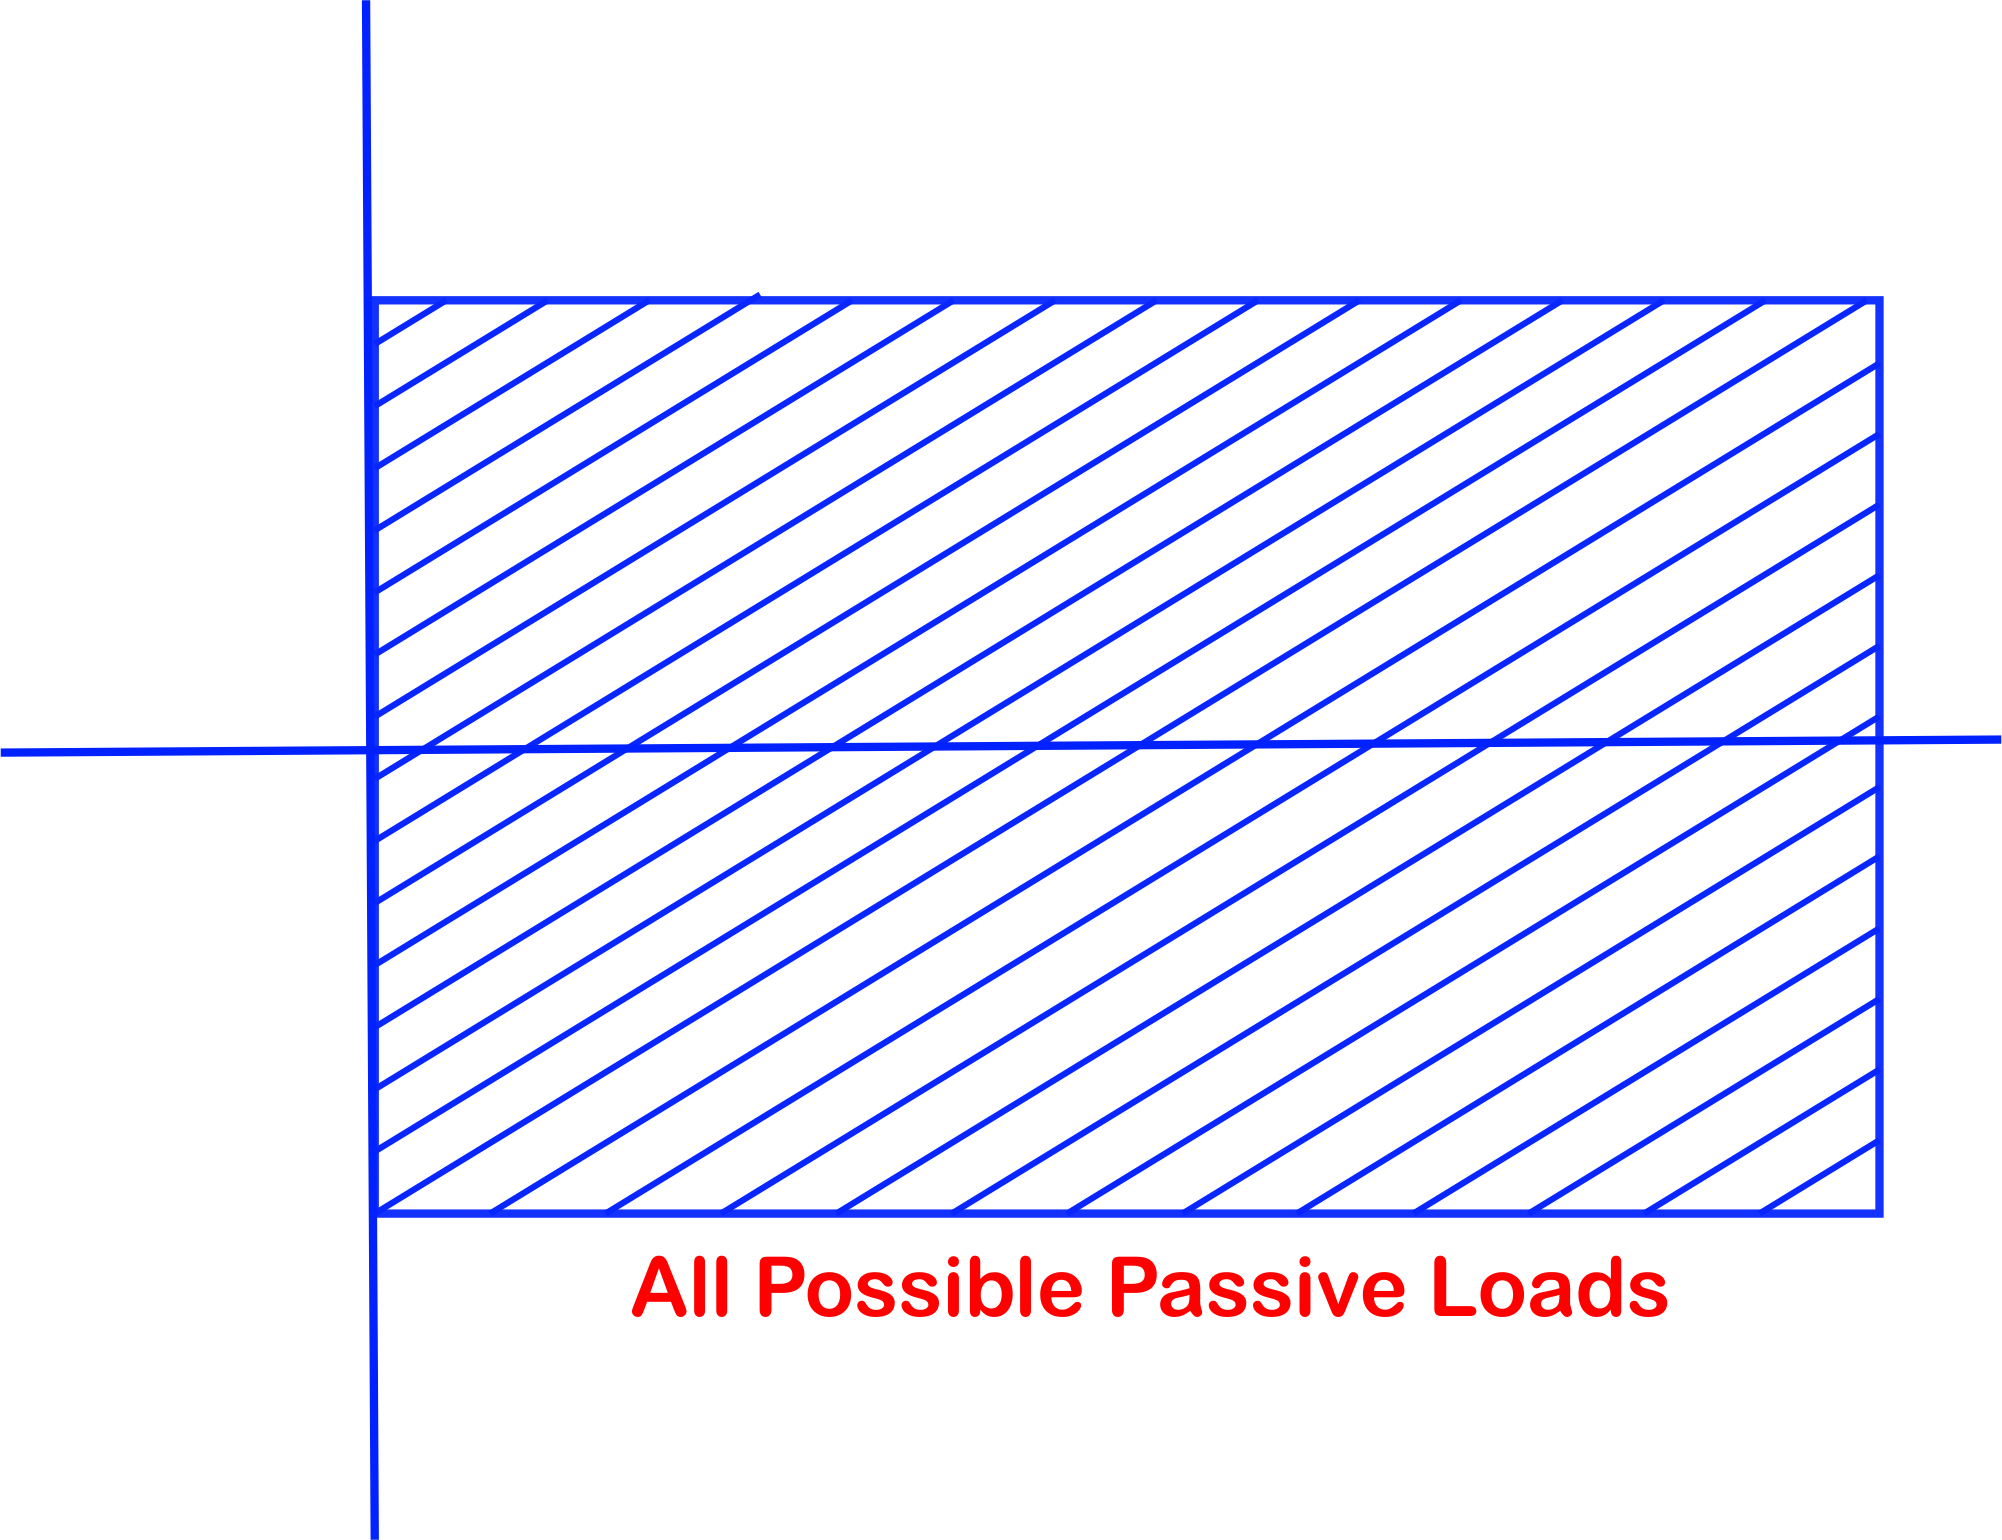
\includegraphics[width=0.6\linewidth]{\pathtopartone/graphics/oigvbnkliu}
\caption{Representation of all passive loads on the complex Z- plane}
\label{fig:oigvbnkliu}
\end{figure}

Solving problems of transmission lines using the z-plane is quite difficult. For this reason, the impedance which was normalized with respect to the characteristic impedance is transformed into another plane which we shall call the \textbf{complex co-efficient plane}\index{complex co-efficient plane} or \textbf{Gamma-plane}\index{gamma-plane} ($\Gamma$).
The transformation from the z-plane to the $\Gamma$-plane is made possible using the one-to-one relationship that exists between the impedance and the reflection co-efficient $\Gamma$ rewritten in  equation~\eqref{eqn:refcoefficientfromload07}
in general the reflection coefficient will have a real and imaginary part. It can be written in either rectangular or polar form. Let the read part of the reflection coefficient be denoted by U and the imaginary part by v

$\Gamma$ = u + jv = \[ re^{j\theta} \] 

in polar form,  

$\Gamma$ = \[ \frac{\bar{Z_L} - 1}{\bar{Z_L} + 1} \] 

shows that we have a one lo one relationship between the reflection coefficient and the normalized impedance. If we know normalized impedance we can find out the reflection coefficient, if we know reflection coefficient, we can find out the normalized impedance.

$\bar{Z_L}$ = \[ \frac{1 + \Gamma}{1 - \Gamma} \] 

So transformation between normalized impedance and reflection coefficient is a one to one relationship. If we plot reflection coefficient for all passive loads as we have seen earlier, for passion load, the magnitude of the reflection coefficient is always less than or equal to 1. At open or closed circuit, $\Gamma$ = 1. For any other impedance n < 1. So if we plot the reflection coefficient into the complex reflection coefficient plane, what we called the complex gamma-plane we have the right half $\bar{Z_L}$-plane mapping into a unit Circle in the gamma-plane. Now er have 2 planes, complex $\bar{Z_L}$-plane and complex gamma plane. Since there is a one to one transformation between these two planes, every point on the $\bar{Z_L}$-plane is mapped to a point on the $\Gamma$-plane. So first exercise we do is to try and map all impedance into the gamma-plane.
\begin{equation}
\Gamma_L = \frac{Z_L - Z_0}{Z_L + Z_0}\label{eqn:refcoefficientfromload07}
\end{equation}
Normalizing we have;
\begin{align*}
\Gamma_L = \frac{\bar{Z_L} - 1}{\bar{Z_L} + 1}\quad\text{or}\quad\bar{Z_L}= \frac{1 + \Gamma}{1 - \Gamma}
\end{align*}
With this transformation relationship, if the \textbf{normalized impedance} is known, we can find the \textbf{reflection coefficient} and vice versa. Hence in general, the reflection coefficient will have a real and imaginary part. It can be written in either rectangular or polar form. Let the real part of the reflection coefficient be denoted by u and the imaginary part by v. $\Gamma$ u + jv = $re^{j\theta}$ in polar form = $\Gamma$ = $\frac{1 + \gamma}{1-\Gamma}$. So transformation between normalized impedance and reflection coefficient is a one to one relationship. If we plot reflection coefficient for all passive load as we have seen earlier, for passive load, the magnitude of the reflection coefficient is always less than or equal to 1 At open or closed circuit $\Gamma$ = 1. For any other impedance, $\Gamma$ < 1. So if we plot the reflection coefficient into the complex reflection coefficient plane, what we called the complex gamma-plane, we have the right half $\bar{Z_L}$-plane mapping into a unit circle in the gamma-plane  as shown in figure~\ref{fig:oiuhgvcx}.
\begin{figure}[h]
\centering
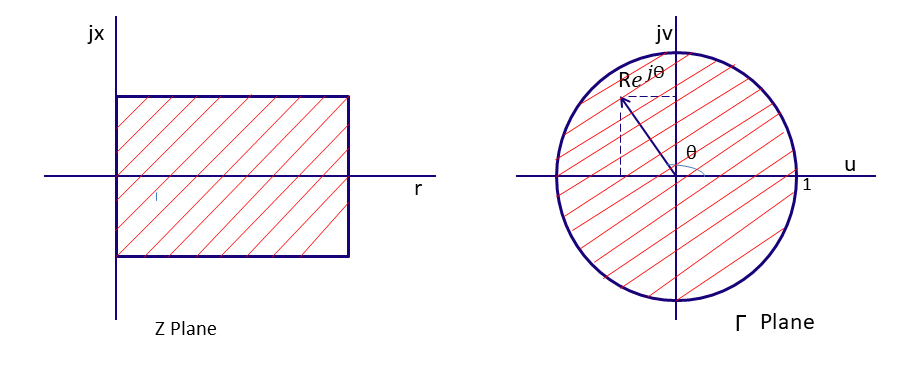
\includegraphics[width=1.05\linewidth]{\pathtopartone/graphics/plane_transform}
\caption{Z-Plane and Complex $\Gamma$-plane}
\label{fig:oiuhgvcx}
\end{figure}

In general, when solving graphically the problems of transmission lines, the basic idea is to take the impedance which is normalized with respect to the characteristics impedance and do a transformation of this impedance into the gamma-plane.

\subsection{Transformation analysis for complex plane}
It was established that since there is a one-to-one transformation between the complex Z-plane and $\Gamma$-plane every point on the Z-plane is mapped to a point on the $ \Gamma$-plane. In this section, we will be \textbf{mapping} the impedance from the Z-plane to the gamma-plane.

Recall, $\bar{Z_L} = r + jx $ and also $\bar{Z_L} = \frac{1 + \Gamma}{1 - \Gamma}$.
\begin{equation}
r + jx =\frac{1 + \Gamma}{1 - \Gamma}
\label{eqn:normequatetransformeqn}
\end{equation}
\begin{equation}
\Gamma\ = u + jv\label{eqn:transformeqn}
\end{equation}
Substituting equation~\ref{eqn:transformeqn} in~\ref{eqn:normequatetransformeqn} we have:
\begin{dmath*}
r + jx = \frac{(1 + u) + jv}{(1 - u) -jv}
= \frac{(1 + u) + jv}{(1 - u) -jv}\times \frac{(1 - u) + jv}{(1 - u) +jv}
=\frac{1 - u^2 + jv(1 + u) + jv(1 - u) - v^2}{{(1 - u)}^2 + jv(1 - u) - jv(1 - u) + v^2}
= \frac{1 - u^2 + 2jv - v^2}{(1 -u)^2 + v^2}
= \frac{1 - (u^2 + v^2) + 2jv}{{(1 - u)}^2 + v^2}
\end{dmath*}
Thus the real and imaginary parts of the equation are:
\begin{align*}
r &= \frac{1 - (u^2 + v^2)}{{(1 - u)}^2 + v^2}\quad\text{(real part)}\\
&\text{and}\\
x &= \frac{2v}{{(1 - u)}^2 + v^2}\quad\text{(imaginary part)}
\end{align*}
Considering the real part, we can express it in the form of the equation of a circle.	
\begin{align*}
r({(1 - u)}^2 + v^2) =& 1 -(u^2 + v^2)\\
r - 2ur + u^2r + v^2r =& 1 - u^2 - v^2\\
u^2(r + 1) -2ur + (r - 1) + v^2(r + 1) =& 0\\
u^2 - 2u\left(\frac{r}{r + 1}\right) + v^2 + \left(\frac{r - 1}{r + 1}\right) =& 0
\end{align*}
We further simplify using the method of completing the squares;
\begin{align*}
{\left(u - \frac{r}{r+1}\right)}^2 + v^2 + \left(\frac{r-1}{r+1}\right) - {\left(\frac{r}{r+1}\right)}^2 = 0
\end{align*}
\begin{align*}
{\left(u - \frac{r}{r + 1}\right)}^2 + v^2 &= {\left(\frac{r}{r + 1}\right)}^2 - \left(\frac{r - 1}{r + 1}\right)\\
{\left(u - \frac{r}{r + 1}\right)}^2+ v^2 &= \frac{r^2 -(r^2 -1)}{{(r + 1)}^2}
\end{align*}
\begin{equation}
{\left(u - \frac{r}{r + 1}\right)}^2+ v^2 = \frac{1}{{(r + 1)}^2}\label{eqn:tranformedresistance}
\end{equation}
Equation~\eqref{eqn:tranformedresistance} represents the equation of a circle in the $uv$ plane centered at $\left(\frac{r}{r + 1}, 0\right) $ with radius $\left(\frac{1}{r + 1}\right)$\footnote{
The general equation of a circle is ${(x - a)}^2 + {(y - b)}^2 = r^2$ where $(a, b)$ are the centre coordinates of the equation and $r$ is the radius.
}.

In a similar way, let's consider the imaginary part.

\begin{equation*}
x = \frac{2v}{{(1 - u)}^2 + v^2}
\end{equation*}
\begin{equation*}
x(1 - 2u + u^2 + v^2) = 2v
\end{equation*}
\begin{equation*}
v^2x - 2v + u^2x - 2ux + x = 0
\end{equation*}

%%\begin{align*}
%%x = \frac{2v}{{(1 - u)}^2 + v^2}\\
%%x(1 - 2u + u^2 + v^2) = 2v\\
%%v^2x - 2v + u^2x - 2ux + x = 0
%%\end{align*}

We divide through by $x$ and factorize
\begin{align*}
v^2 - \frac{2v}{x} +u^2 - 2u + 1 =& 0\\
{(u - 1)}^2 -1 + {\left(v - \frac{1}{x}\right)}^2 -\frac{1}{x^2} + 1 =& 0
\end{align*}
\begin{equation}
{(u - 1)}^2 + {\left(v - \frac{1}{x}\right)}^2 = \frac{1}{x^2}\label{eqn:tranformedreactance}
\end{equation}
Equation~\eqref{eqn:tranformedreactance} represents the equation of a circle in the $uv$ plane centred at $\left(1,\frac{1}{x}\right)$ with radius $\left(\frac{1}{x}\right)$.

From equations~\eqref{eqn:tranformedresistance} and~\eqref{eqn:tranformedreactance}, it can be deduced that for any value of $r$ and $x$, we get a circle on the gamma-plane. The circle that corresponds to \textbf{r} is called the \emph{Circle of Constant Resistance}\index{circle of constant resistance} while the circle that corresponds to $x$ is called the \emph{Circle of Constant Reactance}\index{circle of constant reactance}.

So all point on the circle of constant resistance have same resistance value in the $\bar{Z}$-plane and all point on the constant resistance circle have some reactance in the $\bar{Z}$-plane. we draw these on a gamma-plane taking note of centre and radius for each circle respectively, ($\frac{r}{r + 1}$,0) lie on the real axis in the gamma-plane. For the constant resistance circle, and the radius is $\frac{1}{r + 1}$ and $\Gamma$ varies from 0 to $\infty$. Similarly the constant reactance circle has centre (1,$\frac{}{x}$) i.e, in a vertical line passing the real axis at u = 1 and the radius is $\frac{1}{x}$ and x varies from -$\infty$ to + $\infty$

\subsection{Circle of Constant Resistance}
In order to visualize the plot of the circles of constant resistance we need to transform the limits of the values of $r$, the real part of normalized impedance $\bar{Z_L}$. The limits of $r$ are $[0, \infty]$ both inclusive and thus the corresponding values of the radius of these circles are $[1, 0]$. Plotting the circle for different values of $r$, we get the plot in figure~\ref{fig:ouytre}.
\begin{figure}[h]
\centering
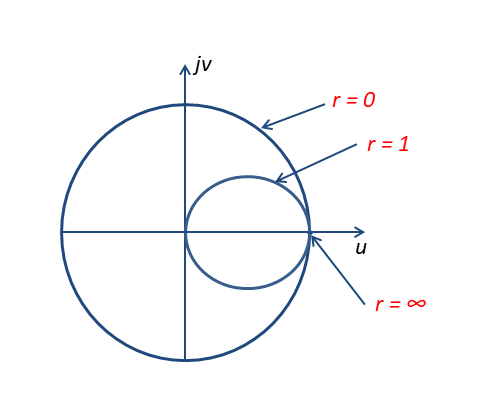
\includegraphics[width=1\linewidth]{\pathtopartone/graphics/fig2.35}
\caption{Plot of the Circles of Constant Resistance at the limits of the values of $r = 0$, $r = 1$ and at $r = \infty$}
\label{fig:ouytre}
\end{figure}

Let's plot for various values of $r$, by varying its value from 0 to $\infty$. At $r = 0$, from equation~\eqref{eqn:tranformedresistance}, the centre of the circle is $(0,0)$ and the radius is 1. At $r = 1$ which is the condition $Z_L = Z_0$ we get the centre at $\left(\frac{1}{2}, 0\right)$ and radius of $\frac{1}{2}$ as shown in figure~\ref{fig:ouytre}.

The complete plot of the circles of constant resistance for the values of increasing $r$ is shown in figure~\ref{fig:rghmgfcx}. It can be said that the centre shifts towards the right and the radius keeps reducing towards zero. At $r = \infty$, the centre is (1,0) and the radius is zero, which is denoted as a dot on the real axis at 1.
\begin{figure}[h]
\centering
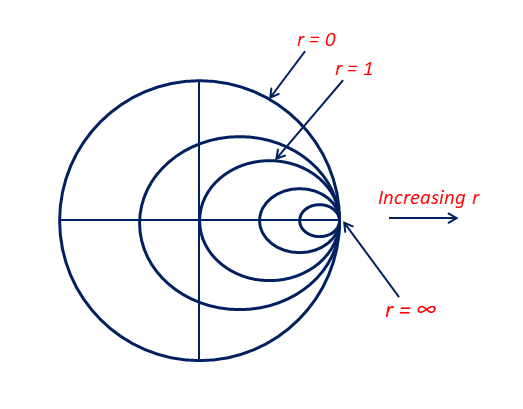
\includegraphics[width=0.9\linewidth]{\pathtopartone/graphics/const_resistance_circles}
\caption{Plot of the circles of constant resistance for increasing values of $r$}
\label{fig:rghmgfcx}
\end{figure}

We can observe that the circles of the constant resistance pass through $u = 1$, and $v = 0$.

\subsection{Circle of Constant Reactance}
Similarly, for the plots of the circles of constant reactance, we consider the limits of the values of $x$ which are $[-\infty, +\infty]$. The corresponding values of the radius of the circle as given by equation~\eqref{eqn:tranformedreactance} are both zero and the radius at $x = 0$ approaches $-\infty$ from the \textbf{negative domain} and $+\infty$ from the \textbf{positive domain} of $x$. Similarly, for the centre \textbf{coordinates} of these circles, considering the negative and positive domains separately, we deduce that the centre of these circles lies on a vertical plane passing through the $u$ axis at $u = 1$ and varies from $-\infty$ to $+\infty$\footnote{
At $x = \pm\infty$, the centre from equation~\eqref{eqn:tranformedreactance} is $(1, 0)$ and at $x = 0$, the centre is $(1, \pm\infty)$.
}.

Figure~\ref{fig:uytrdbn} shows the plot of the circles of constant reactance.
\begin{figure}[h]
\centering
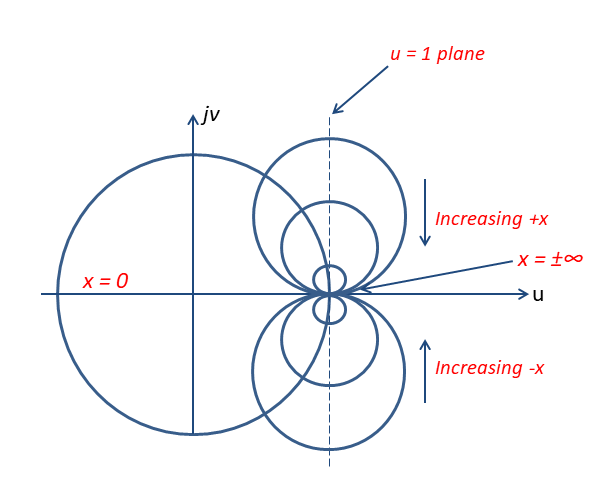
\includegraphics[width=1\linewidth]{\pathtopartone/graphics/plot_of_const_reactance_circles}
\caption{Plot of the circles of constant reactance at the limits $x = \pm\infty$ and $x = 0$ as well as inbetween.}
\label{fig:uytrdbn}
\end{figure}

As seen in figure 2.37, the centre always lies on a line $u = 1$ and as $x$ increases in the \textbf{positive domain}, the centre shifts down along $u = 1$ line and the radius decreases. Similarly, as $x$ increases in the \textbf{negative domain}, the centre shifts up along the $u = 1$ line and the radius decreases. The radius of the circles of constant reactance at $x = 0$ is shown with a line through the origin whose centre is at $\pm\infty$. Also, we can observe that the circles of constant reactance also pass through the coordinate $(u,v) = (1,0)$. This signifies the uniqueness of the point. 

The superimposed plots of the constant resistance and constant reactance circles are thus shown in figures~\ref{fig:ijnbvcxw} and~\ref{fig:sddfghj}.
\begin{figure}[h]
\centering
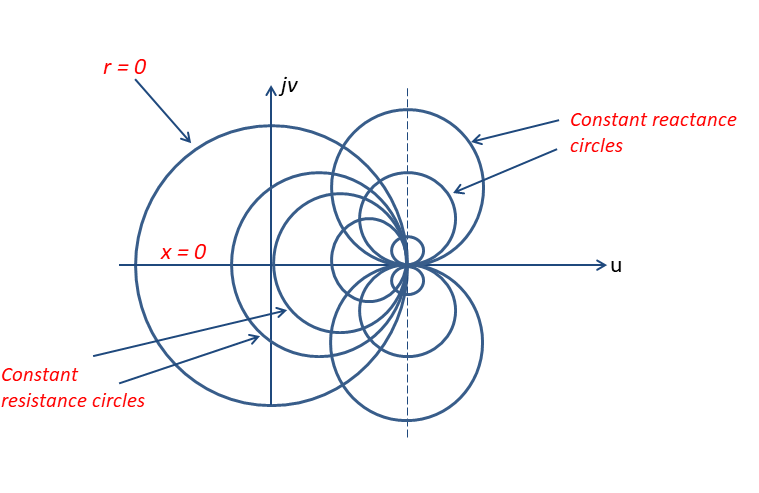
\includegraphics[width=1.1\linewidth]{\pathtopartone/graphics/const_resistance_reactance_circles}
\caption{Plot of the two sets of circles superimposed}
\label{fig:ijnbvcxw}
\end{figure}
\begin{figure}[h]
\centering
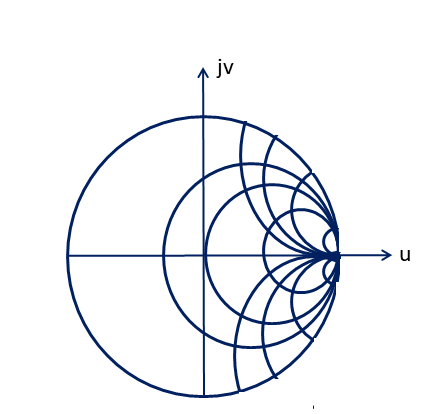
\includegraphics[width=0.8\linewidth]{\pathtopartone/graphics/relevant_region_SC}
\caption{Masking of the superimposed set to relevant region}
\label{fig:sddfghj}
\end{figure}

It can be observed that the superimposed set of circles was masked by the outermost circle with a radius of 1. This circle is called the \textbf{limit circle}\index{limit circle} for the gamma-plane which is the region where $\Gamma\ \leq 1$. This is so because in the analysis of transmission lines, we are not concerned with reflection coefficients that are greater than one, we are only interested in reflection co-efficient that are less than or equal to 1 which is represented by the unit circle of radius of 1 which represent all possible passive loads. It therefore means that any other point outside this range of reflection coefficient, $\Gamma$, is not of practical relevance since it does not represent a passive load. Although the constant reactance circles fill the entire space, we only consider the portion that satisfies $ \Gamma\ \leq 1$ and this lies within the unit circle of the complex gamma-plane.

Some of the observations we made are summarized as follows:
\begin{enumerate}[(i)]
\item All circles of constant resistance have their centre lying on the positive axis and complex gamma-plane.
\item All the circles passes through the point $u = 1$ and $v = 0$.
\item As the value of $r$ increases, the centre of the circles of constant resistance shifts towards the right from the origin to point $u = 1$ and the radius decreases.
\item The centre of the circles of constant reactance circle line in a plane $u = 1$ and the upper half represents the inductive reactance and the lower half capactive reactance.
\item As the reactance value increases in both the positive and negative domain, the centre of the circle shifts towards the right from the origin to  $(1, 0)$ i.e it approaches the u-axis, and the radius of the circle decreases.Similarly, for the constant reactance cirlces, the constant reactance cirlce has a vertical line passing through u = 1 and the upper half represents the positive resistance and the lower half represents the negative reactance
\item When $x = \pm\infty$, the radius of the circle is zero which is a point at $(u,v) = (1,0)$.
\end{enumerate}

\section{The Smith Chart\index{The Smith chart}}
The superposition of the constant resistance circle and the constant reactance circle is now a coordinate system for impedance on the complex gamma-plane. This is called the \emph{Smith chart}\index{smith chart}\footnote{
\centering
\includegraphics[width=0.7\linewidth]{\pathtopartone/graphics/"smith_chart (2)"}
\centering
Figure 2.40: The Complete Smith Chart
}\index{smith chart}. It was developed by PHILIP HAGAR SMITH
\begin{figure}[h]
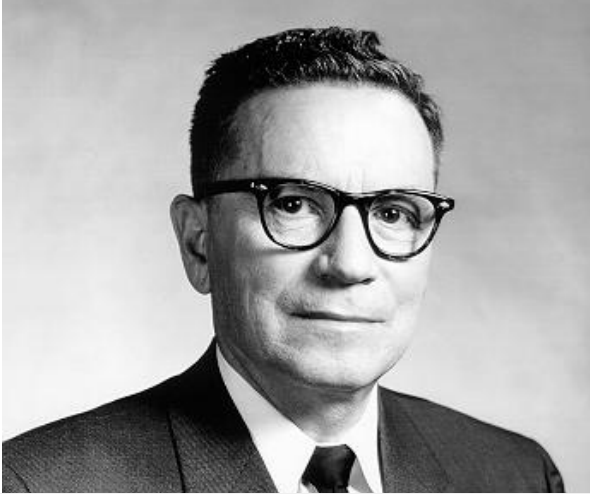
\includegraphics[scale=0.09]{\pathtopartone/graphics/a21}


Philip Hagar Smith (1905-1987), American electrical engineer known for creating the Smith Chart. While at Bell Telephone Labs after graduating from Tufts in 1928, he devised the chart to display and assess various complex impedance parameters, driven by his lifelong passion for graphical math representations. This interest in representing mathematical relationships in graphical form is what led to the invention of the Smith chart.
\label{fig:smithchart-2}
\end{figure}

\textbf{The Smith chart} (shown in figure 2.40 below), is a graphical aid designed for electrical and electronics engineers to assist in solving problems of the transmission lines and matching circuits. It is a product of superimposing the circle of constant resistance and the circle of constant reactance. It can be used to simultaneously display multiple parameters such as the impedances, admittances, reflection coefficient etc.
It is plotted on the complex reflection co-efficient plane in two dimensions and is scaled in normalized impedance (which is most common), normalized admittance or both. It has \textbf{circumstantial scaling} of wavelengths and degrees. The wavelength scale is used in distributed component problems and represents the distance measured along the transmission line connected between the generator and the load to the point under consideration.

Figure~\ref{fig:473-drawingjhgfd} shows the simplified version that will allow us to mark out some important points.
\begin{figure}[h]
\centering
\includegraphics[width=0.7\linewidth]{\pathtopartone/graphics/"473 drawingjhgfd"}
\caption{A Simplified Smith Chart}
\label{fig:473-drawingjhgfd}
\end{figure}

\begin{enumerate}[(i)]
\item The point A or any other point lying on the outermost circle correspond to $r = 0$ while any point lying on the horizontal axis represents $x = 0$

\item The intersection of this horizontal axis and the outermost circle corresponds to $r = 0,x = 0$ at A which is a load that is short-circuited from the impedance point of the line. It, therefore, means that point A is a short circuit.

\item At point B where the two sets of circles disintegrate into, corresponds to $r = \infty$ and $x = \pm\infty $ which is an open circuit.

\item Any point between A and B on the outermost circle represents pure reactances because for these points, r = 0. Above the $u$ axis inside the limit circle, we have the inductive loads, and below the $u$ axis in the limit circle, we have the capacitive loads (it, therefore means we can tell what kind of load we have by where it lies on the Smith chart).

\item At point C where $r = 0$ and $x = +1$, corresponds to purely reactance whose magnitude is equal to the \index{characteristic impedance} of the line.

\item At point D where $r = 0$ and $x = -1$ represent a purely capacitive reactance whose magnitude is equal to the characteristic impedance of the line.

\item The centre of the \index{limit circle} has one more special point M which is the origin of the Smith chart of the gamma-plane is the intersection of $r = 1$ circle and $x = 0$ line.

At M the impedance is equal to the characteristic impedance of the line and that is the point of greatest interest to us because that point represents the \textbf{matched condition} of the transmission line. So when the impedance lies on the centre of the Smith chart, which correspond to the magnitude of the reflection coefficent, $r_L = 0$. This point represent the matched conditon of the transmission line
\end{enumerate}
These points if properly understood can be used to solve transmission line problems with ease.

To solve transmission line problems using the Smith chart, it should be held such that the most clustered portion of the circle should be towards the right hand of the user because the real axis at the complex gamma-plane is in that direction and the complex imaginary plane is in the vertical direction. If done so then calculation on conversion from the complex reflection co-efficient plane to the impedance plane and vice versa can be done easily as well as marking of impedance points on the Smith chart to use to find co-ordinates of the point which gives the reflection co-efficient easily. In conclusion, the Smith chart is a handy tool for solving very complex \index{impedance transformation} problems.


\begin{mdframed}[ backgroundcolor=lightblue, linewidth=1pt, hidealllines=true]
\section*{Exercises}
\begin{ExerciseList}
\Exercise[label={ex32}]
Why do we limit our analysis on the Smith chart to the limit circle?

% \Exercise[label={ex33}]
% As we move along a transmission line, how does a point move on the Smith chart?

\Exercise[label={ex34}]
At what point in solving transmission line problems do we consider the wavelength's scale?

\Exercise[label={ex34}]
Prove mathematically, the one-to-one relationship that is involved in impedance transformation from the ${Z}$-plane to the $\Gamma$\textemdash\;plane.
\end{ExerciseList}
\end{mdframed}
